\documentclass[11pt]{article}

\usepackage[utf8]{inputenc}
\usepackage[T1]{fontenc}
\usepackage{lmodern}
\usepackage{amsmath,amssymb}
\usepackage{graphicx}
\usepackage{booktabs}
\usepackage{array}
\usepackage{xcolor}
\usepackage[margin=1in]{geometry}
\usepackage{tikz}
\usetikzlibrary{arrows.meta,positioning,shapes.geometric}
\usepackage[hidelinks]{hyperref}
\usepackage{microtype}
\usepackage{enumitem}
\usepackage[round]{natbib}
\usepackage{amsthm}
\theoremstyle{definition}
\newtheorem{theorem}{Theorem}
\newtheorem{corollary}{Corollary}
\newtheorem{definition}{Definition}
\newtheorem*{remark}{Remark}

\graphicspath{{../results/figures/}{./figures/}}

\newcommand{\zstar}{\ensuremath{Z^{\star}}}
\newcommand{\code}[1]{\texttt{#1}}
\newcommand{\Exec}{\ensuremath{\mathrm{Exec}}}

% TITLE reframed for the design paper. NOTE: the abstract, introduction, and conclusion prose still
% carry the inverse-compiler framing and are reframed by the queued drafting tasks (intro; abstract
% written last). Sections 3 (manifold) and 6 (design) are in their final design-framed form.
\title{\textbf{Sound Biosynthetic Design over Iterative Grammars:\\A Realizability Geometry for Fungal Polyketides}}

\author{Brage Eilertsen\\
\small \texttt{brageei@uio.no}\\
\small \textit{Affiliation to be completed}}

\date{May 2026}

\begin{document}
\maketitle

\begin{abstract}
Predicting a fungal natural product from its biosynthetic gene cluster (BGC) is usually posed as
direct $\mathrm{BGC}\!\to\!$structure regression, and it stalls---reported balanced accuracies of
$51$--$68\%$, barely moved when a thousand bacterial BGCs are pooled with the few hundred fungal
ones. We argue the regression targets the wrong object. A product is the image
$y=\mathrm{Exec}_{\Theta}(z;G)$ of a latent biosynthetic \emph{program} $z$ executed under an
operator library $\Theta$ and a domain-derived grammar $G$, so the field's ceiling is a statement
about grammar \emph{identifiability}---how much of $z$ the observables pin down---not about how much
data exists. We build a sound inverse compiler over this program space and run it in three
directions. \emph{Forward}, a deterministic executor renders a program to a structure;
\emph{inverse}, a beam verifier returns the exact set $Z^\star$ of legal programs consistent with the
observables, as a typed verdict---\textsc{verified}, \textsc{under-observed} (naming the next
observable that would collapse $Z^\star$), or \textsc{out-of-grammar}. Run inverse across all $326$
fungal PKS in MIBiG~4.0, exact reconstruction reaches $8/326$---not a disappointment but the
\emph{boundary} of the natural manifold the engine operates over (a tailoring-latent reformulation
recovers $64\%$ conditional on a producible core)---and a cross-taxa transfer probe locates its one
hard axis: per-cycle reduction chemistry transfers at $1.00$ within a fixed domain set but collapses
to $0.567$ across the iteration program---bacterial modular and fungal iterative PKS thus instantiate two
computational regimes of catalytic control: \emph{externalized} per-step state (one module per step,
learnable) versus \emph{compressed}, state-dependent routing through one reusable manifold.

Run \emph{backward}, the same engine becomes a design tool. We place a desired molecule on a
\emph{realizability geometry} against the natural manifold, decomposed onto two axes that map to
different wet-lab capabilities---\emph{structural} edits (domain content; mature bacterial
modular-PKS precedent) and \emph{control} edits (the iteration program; the $0.567$ frontier)---scored
by a literature-curated, super-additive cost that \emph{is} the field's measured engineering
difficulty rather than an assumption we supply. Across the $1$-edit neighbourhood of the manifold the
control axis dominates ($69$ frontier to $49$ engineerable), and an experiment-selection planner
ranks the observation that would most collapse $Z^\star$ per unit cost. The same iteration-grammar
wall is thus a prediction ceiling read one way and a design frontier read the other---a symmetry we
formalise as an \emph{identifiability--controllability duality} (Theorem~\ref{thm:duality},
\S\ref{sec:duality}): the verifier's consistent set and the designer's specification space are one
equivalence class, so prediction and design ambiguity are projections of a single observability quantity
$\kappa_O$, a result that travels beyond fungal PKS with a falsifiable prediction on RiPP biosynthesis.
Because structure elucidation in this field proceeds by heterologous expression and NMR with mass
spectrometry as triage---the methodology of all seven verified products we curate from primary
sources---we build a metabologenomics \emph{triage} tool whose three-state verdict names explicitly
the clusters where triage suffices and those that must go to expression$+$NMR. The observability and
verdict layers are family-agnostic, demonstrated unchanged over PKS, a non-ribosomal peptide (NRPS)
grammar, and a typed PKS--NRPS hybrid; only the program generator is family-specific. All tools,
data, and analyses are open and reproducible from single commands.
\end{abstract}

\section{Introduction}\label{sec:intro}

Many fungal drugs---the cholesterol-lowering agent lovastatin, the antifungal griseofulvin---are
polyketides: large carbon scaffolds assembled by a multidomain enzymatic factory, the polyketide
synthase (PKS), encoded by a contiguous biosynthetic gene cluster (BGC). Genome
sequencing has revealed that filamentous fungi carry vast numbers of such clusters, most of
them \emph{cryptic}: no metabolite has ever been linked to them. They are widely regarded as
one of the most promising untapped reservoirs of new bioactive chemistry.

Turning a cryptic fungal BGC into a candidate molecule requires answering: \emph{what} would
the cluster make? Recent machine learning has attacked this with limited success.
\citet{riedling2024} trained classical classifiers to predict the bioactivity class of fungal
secondary metabolites from BGC features; trained on $314$ fungal BGCs they reached balanced
accuracies of $51$--$68\%$, and adding $1{,}003$ bacterial BGCs moved this only to
$56$--$68\%$. That second result is our point of departure: if the bottleneck were a shortage
of fungal examples, a fourfold increase in (cross-domain) training data should help
substantially. It did not. (The two ceilings measure different quantities---\citet{riedling2024}
classify bioactivity, we reconstruct structure---but we argue both reflect the same grammar
mismatch, and we draw no direct numerical comparison.)

The deeper issue is the framing. \emph{Natural-product discovery should not be posed as direct
$\mathrm{BGC}\!\to\!$structure regression, but as verifier-grounded inference over---and design
upon---latent biosynthetic programs constrained by genome-derived grammars and physical
observables.} A BGC is not a molecular blueprint but a constrained program space: the product is the
image $y=\mathrm{Exec}_{\Theta}(z;G)$ of a latent program $z$ under a biochemical operator library
$\Theta$ and a domain-derived grammar $G$. We realize this as a \textbf{grammar-agnostic biosynthetic
inverse compiler} (Figure~\ref{fig:arch}) and run it in three directions on one spine: a
grammar-specific executor enumerates legal programs \emph{forward}; a shared observability layer and
verifier collapse them against mass and MS/MS \emph{inverse}, returning a three-state verdict; and
run \emph{backward}, the same grammar places a desired molecule on a realizability geometry against
the natural manifold and ranks the experiments that would confirm it (Section~\ref{sec:design}). In
this sense the framework is \emph{neuro-symbolic}: symbolic execution and verification enforce mass
balance, legal reaction structure, and observable consistency, while learned models are reserved for
the genuinely high-dimensional pieces---sequence-dependent activity, stereochemistry, and hidden
transition policies. More than a predictor, the executor is then a \emph{substrate on which other
models compose soundly}: a learned sequence policy can rerank within the legal set $Z^{\star}$, a
bioactivity model can filter it, and wet-lab build outcomes can update the realization cost---each
inheriting the executor's soundness rather than eroding it. This is the middle the field lacks:
generative chemistry yields molecules with no construction plan or feasibility guarantee,
retrosynthesis searches reactions to commercial reagents but ignores enzyme space, and genome mining
asks only what nature already makes. An executable, cost-weighted definition of biosynthetically
realizable space---each point carrying a construction program $z$ and a verifying observable---is what
a \emph{target-directed} search over makeable chemistry requires. This stance answers a field
diagnosis rather than ignoring it: Cox's review of
iterative highly-reducing PKS programming finds it an emergent property and rational engineering
``extremely difficult,'' naming machine learning as the way forward \citep{cox2023}---which we read
as a design \emph{constraint}, not an endorsement, requiring the architecture to stay \emph{sound}
precisely where rational reprogramming is intractable. We also scope the contribution honestly:
structure elucidation in this field proceeds through heterologous expression and NMR with mass
spectrometry as triage, so we build a metabologenomics \emph{triage} tool grounded in those
observables that names explicitly the clusters where triage is insufficient and structure
elucidation is required. We do \emph{not} claim a complete genome-to-structure predictor or a
replacement for structure elucidation; we contribute the architecture, a characterization of the
natural manifold that explains the field's ceiling, a realizability geometry that turns the same
engine into a design tool, and cross-grammar demonstrations. Our contributions are:

\begin{enumerate}[leftmargin=1.4em,itemsep=2pt]
\item A \textbf{grammar-agnostic inverse compiler} over biosynthetic program grammars: a sound
deterministic executor and beam verifier returning the exact consistent program set \zstar{}
behind one observable-constrained interface (Sections~\ref{sec:executor}--\ref{sec:verifier}).
\item A \textbf{deterministic reconstructibility analysis} of fungal iterative PKS over MIBiG~4.0
(Section~\ref{sec:manifold}): exact-match $8/326$, a core-match \emph{sensitivity} showing
structural-similarity proxies are unreliable, and a tailoring-latent reformulation ($7/106$;
$64\%$ conditional on a producible core), with a curated literature benchmark
(Section~\ref{sec:benchmark}) and a cross-taxa transfer probe of the iteration-grammar wall
(Section~\ref{sec:manifold}).
\item A \textbf{shared metabolomics observability layer} (Section~\ref{sec:mining}): an
adduct-aware, ppm-tolerant approximate verifier $Z^{\star}_{\epsilon}$, a within-grammar
formula-ambiguity report, a tolerance-scored MS/MS matcher, and a minimum-sufficient-observables
planner.
\item \textbf{Cross-grammar demonstrations} on PKS, NRPS, and a typed PKS--NRPS hybrid bridge
(Section~\ref{sec:crossgrammar})---the same observability and verdict layers, only the program
generator changing.
\item A \textbf{realizability geometry for biosynthetic design} (Section~\ref{sec:design}): every
target molecule scored by its edit distance to the natural manifold on two typed axes---%
\emph{structural} (domain content, with bacterial modular-PKS precedent) and \emph{control} (the
iteration program, the $0.567$ frontier)---under a \emph{literature-curated, super-additive} cost that
encodes the field's measured engineering difficulty, with a worked design neighbourhood, the
control-axis dominance result ($69\!:\!49$), and an \textbf{experiment-selection planner} that ranks
the next observation by expected collapse of $Z^\star$ per unit cost and names the
elucidation-required designs.
\item An \textbf{identifiability--controllability duality} (Theorem~\ref{thm:duality},
\S\ref{sec:duality}): the inference resolution $Z^{\star}$ and the design resolution $D(y;O)$ are the
same equivalence class $[z]_O$, so prediction ambiguity and design specification freedom are one
quantity $\kappa_O$ at one observability frontier $\mathcal{F}_O$; instantiated on PKS, NRPS, and hybrid
grammars and predicted to survive on RiPP (Corollary~\ref{cor:crossfamily}).
\item A \textbf{three-state reconstructibility verdict} (\textsc{verified} / \textsc{under-observed}
/ \textsc{out-of-grammar}) in which the \textsc{under-observed} state names the next observable that
would collapse $Z^\star$, resting on a failure-mode taxonomy (operator coverage, hidden iterative
control, tailoring under-constraint, non-local structure) that replaces a single accuracy score.
\end{enumerate}

\begin{figure}[t]
\centering
\resizebox{\linewidth}{!}{%
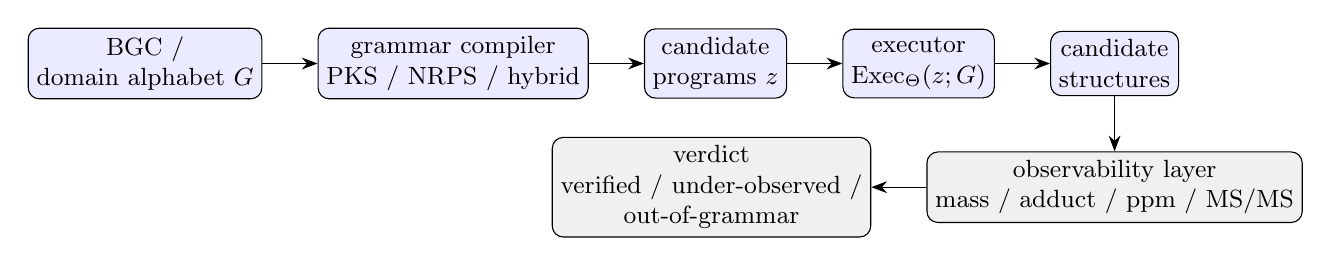
\begin{tikzpicture}[node distance=4mm and 7mm,
  box/.style={draw,rounded corners,align=center,inner sep=3pt,minimum height=8mm,font=\small},
  fam/.style={fill=blue!8}, sh/.style={fill=gray!12},
  >={Stealth[length=2mm]}]
\node[box,fam] (bgc) {BGC /\\domain alphabet $G$};
\node[box,fam,right=of bgc] (gram) {grammar compiler\\PKS / NRPS / hybrid};
\node[box,fam,right=of gram] (prog) {candidate\\programs $z$};
\node[box,fam,right=of prog] (exec) {executor\\$\mathrm{Exec}_\Theta(z;G)$};
\node[box,fam,right=of exec] (struct) {candidate\\structures};
\node[box,sh,below=7mm of struct] (obs) {observability layer\\mass / adduct / ppm / MS/MS};
\node[box,sh,left=of obs] (verd) {verdict\\verified / under-observed /\\out-of-grammar};
\draw[->](bgc)--(gram); \draw[->](gram)--(prog); \draw[->](prog)--(exec); \draw[->](exec)--(struct);
\draw[->](struct)--(obs); \draw[->](obs)--(verd);
\end{tikzpicture}}
\caption{The grammar-agnostic inverse compiler. Family-specific grammars (blue) compile a cluster's
domain alphabet into candidate programs that a sound executor renders to structures; a shared
observability layer (grey) collapses the candidate set with mass and MS/MS, and a shared verifier
returns a three-state reconstructibility verdict. Only the grammar and executor are family-specific;
the observability and verdict layers are reused across PKS, NRPS, and hybrid grammars.}
\label{fig:arch}
\end{figure}

All numbers in this paper are produced by the open code base by a single documented command
and are traceable to a git commit; Appendix~\ref{app:repro} lists the commands.

\section{Background and the grammar-mismatch hypothesis}
\label{sec:background}

\paragraph{Modular vs.\ iterative assembly lines.} Bacterial type~I modular PKS---the
archetype being the 6-deoxyerythronolide~B synthase---are \emph{colinear}. Each elongation
module carries its own ketosynthase (KS) and acyltransferase (AT) for chain extension and an
optional reductive cassette of ketoreductase (KR), dehydratase (DH) and enoylreductase (ER).
The final product can be read off the linear order of modules. This clean structure-to-function
map is why rule-based detectors such as antiSMASH \citep{antismash} and PRISM
\citep{prism} and the design database ClusterCAD \citep{clustercad,clustercad2} perform well
on bacteria.

Fungal PKS are overwhelmingly \emph{iterative}: a single set of catalytic domains is reused
across $N$ cycles, and which reductive steps fire on which cycle is governed by a program that
no current tool decodes. The highly-reducing (HR), non-reducing (NR) and partially-reducing
(PR) subclasses behave like distinct programming languages. The lovastatin nonaketide synthase
LovB runs eight cycles with a different reduction state each time, and its own ER domain is
degenerate---ER activity is supplied \emph{in trans} by the standalone partner LovC
\citep{ma2009}. In NR-PKS a dedicated product-template (PT) domain dictates the regioselectivity
of aromatic-ring cyclization \citep{crawford2009}.

\paragraph{The hypothesis, sharpened to reconstructibility.} We hypothesize that the $51$--$68\%$
ceiling reflects a control-flow mismatch rather than a sample-size limit. We state this as a
\emph{reconstructibility} (identifiability) property, not undecidability: throughout, ``computable''
is shorthand for whether the per-step core is recoverable from the BGC-visible domain content under
our sound executor grammar. In colinear assembly lines the per-step core \emph{is a
function of domain content} and can therefore be tabulated (ClusterCAD); in iterative assembly
lines the same domain set must perform different chemistry on different cycles, so the per-step
core is \emph{not} a function of domain content and the end-product-to-program map is
many-to-one and unobserved. A model trained on colinear data learns a control flow that is not
merely uninformative but incorrect for fungi---the near-flat cross-domain result of
\citet{riedling2024} is exactly the prediction this hypothesis makes. The rest of this paper
turns the hypothesis into measurements.

\section{A verifier-grounded executor}
\label{sec:executor}

We represent the product of an iterative synthase as the output of a discrete latent
\emph{program} executed by a sound, deterministic chemical executor (Figure~\ref{fig:pipeline}).
A program is an ordered list of catalytic cycles,
\begin{equation}
z = \big\{(c_t, a_t)\big\}_{t=1}^{N},
\end{equation}
where $c_t$ marks a chain-elongation event and $a_t$ is an action over the reductive cascade
and tailoring chemistry. The cascade is strictly ordered---ER presupposes DH presupposes
KR---giving the four reachable $\beta$-states (keto, hydroxyl, enoyl, methylene) plus an
optional $\alpha$-methylation (C-MeT) and a terminal chain release. The executor renders a
program into a molecule, $\hat y = \mathrm{exec}(z)$.

\paragraph{Deterministic core, not weights.} Each operator is a fixed reaction encoded as a
reaction SMARTS and applied with RDKit \citep{rdkit}: a decarboxylative Claisen condensation
appends a $\mathrm{C}_2$ ketide unit; KR reduces the $\beta$-ketothioester to the
$\beta$-hydroxy; DH eliminates to the enoyl; ER reduces to the methylene; C-MeT
$\alpha$-methylates; the thioesterase/cyclase releases the chain. The growing chain is modelled
as an ACP-tethered thioester whose carrier is a single sentinel atom, so the unique active
thioester anchors every operator unambiguously. The core is \emph{validated}, not trained: we
confirm each operator by exact mass bookkeeping (extension $+\mathrm{C_2H_2O}$, KR $+\mathrm{H_2}$,
DH $-\mathrm{H_2O}$, ER $+\mathrm{H_2}$, C-MeT $+\mathrm{CH_2}$) and by reconstructing known
polyketides. Single-mode cyclization---lactonization, the small-aromatic aldol (orsellinic,
6-MSA) and the mellein dihydroisocoumarin---is implemented; the five-class PT-domain
regiochemistry of large NR-PKS and the lovastatin Diels--Alder are deliberately scoped out and
flagged. The executor is a pure, deterministic function validated within the project's regression
suite ($116$ tests).

\begin{figure}[t]
\centering
\resizebox{\linewidth}{!}{%
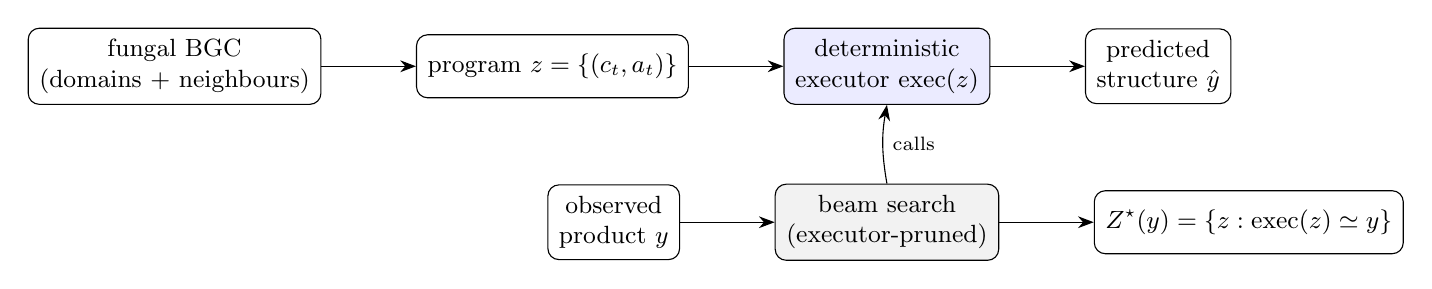
\begin{tikzpicture}[node distance=6mm and 12mm,
  box/.style={draw,rounded corners,align=center,inner sep=4pt,minimum height=8mm,font=\small},
  >={Stealth[length=2mm]}]
\node[box] (bgc) {fungal BGC\\(domains $+$ neighbours)};
\node[box,right=of bgc] (prog) {program $z=\{(c_t,a_t)\}$};
\node[box,right=of prog,fill=blue!8] (exec) {deterministic\\executor $\mathrm{exec}(z)$};
\node[box,right=of exec] (yhat) {predicted\\structure $\hat y$};
\node[box,below=10mm of exec,fill=gray!10] (beam) {beam search\\(executor-pruned)};
\node[box,left=of beam] (y) {observed\\product $y$};
\node[box,right=of beam] (zstar) {$Z^{\star}(y)=\{z:\mathrm{exec}(z)\simeq y\}$};
\draw[->] (bgc)--(prog); \draw[->] (prog)--(exec); \draw[->] (exec)--(yhat);
\draw[->] (y)--(beam); \draw[->] (beam)--(zstar);
\draw[->] (beam.north) to[bend left=10] node[right,font=\scriptsize]{calls} (exec.south);
\end{tikzpicture}}
\caption{The executor (top) renders a program to a structure; the verifier (bottom)
inverts it by beam-searching programs, executing each candidate and pruning any whose partial
product cannot reach $y$, returning the exact consistent set \zstar{}.}
\label{fig:pipeline}
\end{figure}

\section{The verifier and identifiability}
\label{sec:verifier}

Because the executor is sound and deterministic and the program space is small ($N$ typically
$4$--$10$, roughly eight admissible actions per cycle), we recover programs by enumeration
rather than amortized inference. Given a target $y$ and an operator set, a beam search emits
programs, executes each (partial) program, and prunes any whose partial product cannot reach
$y$. We accept a program into the \emph{verified consistent set}
\begin{equation}
\zstar = \big\{\, z : \mathrm{exec}(z) \simeq y \,\big\},
\end{equation}
where $\simeq$ is graph isomorphism up to canonicalization. Two prunes make the search cheap: a
carbon-count bound and an \emph{analytic molecular-formula} prefilter that computes a program's
released-acid formula from validated per-cycle deltas and only executes formula-consistent
candidates (e.g.\ this takes the mellein search from $1{,}792$ to $93$ executor calls).

\paragraph{Validation and identifiability.} On the curated benchmark the known program is
contained in \zstar{} for all systems, and the search is deterministic and fast (mean
$0.28$\,s/target). Observed degeneracy on the curated set is $|\zstar|=1$: programs are
identifiable at these chain lengths. Genuine degeneracy \emph{is} detectable when the operator
set permits an alternative route---e.g.\ hexanoic acid is reached as
$\text{acetyl}+2\!\times\!\text{ER}$ or $\text{butyryl}+1\!\times\!\text{ER}$, giving
$|\zstar|=2$---so identifiability is governed by the operator-set constraints, as the
formulation predicts.

\subsection{Guarantees}
\label{sec:guarantees}
All guarantees are stated relative to the operator library $\Theta$, the (domain-derived) grammar
$G$, the observable set $O$, and---for the tolerant mass observable (Section~\ref{sec:mining})---the
mass tolerance $\epsilon$ and the adduct model. For
$Z^{\star}_{\Theta}(y;G,O)=\{\,z\in Z_{\Theta}(G,O):\mathrm{Exec}_{\Theta}(z;G)\simeq y\,\}$
the search is \emph{sound}---every returned $z$ executes to a structure matching $y$ under
$\simeq$---and \emph{relatively complete}: every legal program in the enumerated grammar that
matches $y$ is returned, up to the beam bound. It is deliberately \emph{not} biologically complete:
if nature uses an operator outside $\Theta$, an empty $Z^{\star}$ is correct relative to $\Theta$
even though the molecule is producible \emph{in vivo}. An empty consistent set is therefore a typed
\emph{certificate of failure mode}---missing operator, hidden control, tailoring under-constraint,
or non-local pathway---not a claim of biological impossibility; the approximate verifier
$Z^{\star}_{\epsilon}$ inherits the same relativity, now also to $\epsilon$ and the allowed adducts.
Because the operator library is modular, extending the engine to complex polycyclic cascades,
trans-acting tailoring events, or additional release chemistries does not require changing the
shared verifier or observability layers; it requires registering new typed operators in the
relevant family-specific executor.

\section{A curated benchmark of fungal PKS programs}
\label{sec:benchmark}

We hand-curate twelve literature-sourced fungal polyketide programs (Table~\ref{tab:bench}),
each a machine-readable specification of starter, per-cycle reduction/methylation, and release,
with a literature citation, a provenance tag (\emph{independent} ground truth vs.\ \emph{pending}
an authoritative structure), and a confidence flag. Six gate-tier entries with independent
ground truth round-trip exactly through the executor; sanity entries cover the reductive
extremes; harder systems (the LovB nonaketide; the TenS PKS--NRPS backbone) are retained as
trace-level assets.

A finding from curation is worth stating: the executor caught a mass-balance inconsistency in a
literature-pass program for mellein. The single-ketoreduction program reconstructs
6-hydroxymellein ($\mathrm{C_{10}H_{10}O_4}$), not mellein ($\mathrm{C_{10}H_{10}O_3}$); mellein
requires a \emph{second} ketoreduction. The verifier earns its keep by making such errors
impossible to overlook.

\begin{table}[t]
\centering\small
\caption{Curated benchmark (excerpt). Reduction states: K keto, H hydroxyl, E enoyl, M
methylene. Gate-tier entries round-trip exactly through the executor.}
\label{tab:bench}
\begin{tabular}{@{}llll@{}}
\toprule
System & Subclass & Program (starter $+$ cycles) & Tier \\
\midrule
Triacetic acid lactone & NR & acetyl $+$ K,K $\to$ lactone & gate (sanity) \\
Orsellinic acid        & NR & acetyl $+$ K,K,K $\to$ aldol  & gate \\
6-Methylsalicylic acid & PR & acetyl $+$ K,H,K $\to$ aldol  & gate \\
Mellein                & PR & acetyl $+$ H,K,H,K $\to$ dihydroisocoumarin & gate \\
6-Hydroxymellein       & PR & acetyl $+$ H,K,K,K $\to$ dihydroisocoumarin & gate \\
2-Methylbutyric acid (LovF) & HR & acetyl $+$ M$_{\text{+Me}}$ & gate \\
LovB nonaketide        & HR & acetyl $+$ 8 cycles ($+$DA) & hard / Phase-2 \\
Tenellin backbone (TenS) & HR & acetyl $+$ 4 cycles ($+$NRPS) & Phase-2 trace \\
\bottomrule
\end{tabular}
\end{table}

% --- §3 (characterizing the manifold) supersedes the old three-tier reconstruction and the
% "grammar mismatch is the data deficit" sections; the wall decomposition and the conceptual
% result are folded into the manifold characterization. ---
\section{Characterizing the natural manifold}\label{sec:manifold}

The natural fungal PKS manifold has \textbf{nine exactly-reachable cores}, a \textbf{0.567 control-axis
ceiling with a structural mechanistic explanation}, an \textbf{interior whose residual hardness sits on
the core, not the tailoring}, and---characterizing the out-of-grammar remainder---a
\textbf{corpus-wide coverage census} that sorts each gap onto a sound-expressibility ladder
(\S\ref{sec:census}) --- this section characterizes its shape. We read these results not as a
catalogue of where prediction fails but as the geometry the design contribution of \S\ref{sec:design}
operates over: the boundary of what nature builds, the axis along which it is hard to read, and the
interior, where decorations are near-uniquely recovered once a core is in hand.

\subsection{The boundary: nine exactly-reachable cores}\label{sec:boundary}
The natural manifold has \textbf{nine exactly-reachable cores}, defining its boundary: of the 326 fungal
PKS entries in MIBiG~4.0, exactly nine are placed exactly by the sound grammar run inverse. That placement is a statement about
\emph{structure}; at the finer grain of the \emph{program} the scan pins eight of the nine to a unique
route ($|Z^{\star}|{=}1$, \textsc{verified}), while the ninth---olivetolic acid---is reached as a structure
but admits two sound programs at one formula ($|Z^{\star}|{=}2$, program-\textsc{under-observed}). The two
routes render the \emph{identical} structure, so no product observable separates them: the degeneracy is
resolved by the genome-read starter/loading domain, not by any product measurement
(Table~\ref{tab:crossgrammar}'s collapse to one is \emph{structure}-level, under a different $(\Theta,O)$). Reach is thus $9$
(structures placed) and program-verified $8$ (routes pinned)---a structure-versus-program distinction of
granularity, not a smaller boundary. This count is
a lower bound \emph{in principle}---some missing operators are enumerable, so coverage could move it
up---but the census of \S\ref{sec:census} shows that increment is zero for sound, no-new-regiochemistry
extension (olivetolic acid, the one such core, is now among the reachable nine), the rest gated on
operators whose soundness is unproven (\S\ref{sec:limits}); it is a
\emph{boundary condition}, not an accuracy: the
set of cores the current sound grammar places exactly, the edge from which \S\ref{sec:design} measures
design distance. ``Only 9'' is the wrong frame; ``the manifold's boundary is here, and it is sharp'' is
the right one.

\subsection{The coverage census: the boundary is genuine, and the remainder is mostly entangled}
\label{sec:census}
The nine is a \emph{boundary} only if the unreached remainder is genuinely out of grammar rather than
merely unscanned, and a \emph{useful} boundary only if we can say what \emph{kind} of operator each gap
needs. Both are settled over the full $326$ (tables in Appendix~\ref{app:census}). \textbf{The partition:}
nine cores are reachable; $205$ are CHO chemistry a polyketide grammar could in principle reach (the
\emph{in-scope} gap); $112$ carry non-CHO atoms (N, halogen, S) and belong to a different grammar
(NRPS-hybrid / halogenase --- a \emph{scope boundary}, not a coverage failure), nitrogen dominating
($98$ of $112$). \textbf{The boundary is not a scan artifact:} the reachability search caps at
$C{\le}20$ for tractability, so re-scanning all $94$ larger cores with the cap lifted to $C80$ reached
\emph{zero} of the $91$ conclusively tested (three exhausted the reduced budget, held inconclusive). The
size cap was concealing no reachable core, so $9/326$ is a real boundary of the grammar's reach, not a
tractability limit --- which forecloses the most immediate objection to ``only nine.'' \textbf{The
in-scope remainder is mostly entangled:} a structural-proxy set-cover --- an explicit \emph{upper bound}
on recovery, since a core counts as proxy-recovered when all its tagged operator classes are present
(necessary, not sufficient) --- is concentrated into a few coarse families but dominated by
non-aromatic-ring/macrolactonization ($176/205$), not aromatic cyclization, and overwhelmingly
entangled: $178$ of the $205$ in-scope cores ($87\%$) touch a family whose sound expressibility is
unproven (\S\ref{sec:limits}), and sound extension with \emph{no} new regiochemistry adds no further
buildable core beyond the nine: the one clean single-class aromatic an already-encoded closure reaches
--- olivetolic acid, whose $\beta$-resorcylic core the generalized C2$\to$C7 closure builds (now among
the reachable nine, the \textsc{verified} cross-grammar build of Table~\ref{tab:crossgrammar}) --- is
already inside the boundary, and the other clean aromatics need PT closures not yet encoded (new
regiochemistry). So ``coverage moves the nine up'' is true in principle yet empty in practice today for
sound, no-new-regiochemistry extension: the gain is zero, and the rest is the located research problem
of \S\ref{sec:limits}, not scheduled
engineering.

\subsection{Similarity is not a reconstructibility metric}\label{sec:proxy}
A natural temptation is to soften the boundary with a structural-similarity proxy --- count a core
``reconstructed'' if a predicted skeleton embeds in the product. We show this proxy is \emph{unreliable}:
it swings from 9 to 160 reconstructed cores as a single nuisance parameter (the allowed ring-closure
slack) is varied, and it admits non-PKS false positives (a de-heteroatomed alkaloid skeleton can embed in
a polyketide chain). Similarity is therefore not a reconstructibility metric; we keep exact match as the
airtight signal and use the tailoring-latent reformulation below as the principled relaxation, not a
tunable proxy.

\subsection{The interior: bounded by core reachability}\label{sec:interior}
Most MIBiG products are a PKS core plus post-PKS tailoring, so exact core-match understates
reconstructibility. Moving tailoring into the latent --- $z=(z_{\mathrm{PKS}},z_{\mathrm{tail}})$ with a
gene- and formula-budgeted edit applier --- the joint search exactly reconstructs \textbf{7/107}
annotated clusters (whole products including tailoring; a different target and denominator from the
\emph{nine} exact cores over all $326$, \S\ref{sec:boundary}). Two reproducible facts shape the interior:
only $9/326$ cores are built exactly (\S\ref{sec:boundary}), and wherever a core is producible the
tailoring search verifies near-uniquely (small $|Z^{\star}|$). The residual hardness therefore sits on
core cyclization, with tailoring near-unique once a core is in hand.

\subsection{The hard axis: the iteration-grammar wall, structurally explained}\label{sec:wall}
The manifold's one genuinely hard axis is per-cycle control. A cross-taxa transfer probe makes it
quantitative: the per-step reduction chemistry is learnable from abundant bacterial modular data and
transfers to fungal cycles \emph{perfectly} when each cycle's active reductive domains are given
($1.00$), but collapses to \textbf{0.567} when only the synthase's fixed domain set is given --- the
iteration-grammar wall. The wall decomposes into a narrow highly-reducing per-cycle-reduction control wall
($\sim$9\% of products) and a broad, coverage-addressable aromatic-cyclization wall ($\sim$61\%).

\paragraph{Why the wall is structural, not a data gap.} A fungal iterative synthase reuses one set of
catalytic domains across every cycle; the per-cycle outcome is fixed by the chain-length and substrate
context the enzyme sees on that pass, not by any per-cycle change in the (constant) machinery. This is the
precise form of Cox's observation that highly-reducing PKS programming is an emergent property that
``will remain extremely difficult'' to predict rationally \citep{cox2023}: it is emergent from the
interaction between the constant catalytic machinery and the changing substrate context across cycles. The
0.567 is therefore not a placeholder for missing work; it is a structural ceiling for any predictor whose
input is the synthase's fixed domain content. A positive/negative control on the same predictor isolates
this. Over 141 colinear bacterial clusters, predicting each module's reduction from its \emph{own}
per-module domains reaches \textbf{0.78}; predicting it from the synthase's single \emph{pooled} domain
set---the condition a fungal iterative synthase is in by construction---collapses to \textbf{0.50} (the
modal baseline), and the fungal $0.567$ sits in that pooled column. One predictor nearly doubles when
given a per-step signal and falls to the wall when denied it: the deficit is the missing per-step
\emph{input}, not the model. (Whole-program exact recovery is only $0.17$ even on bacteria, as per-module
errors compound across the assembly line---which is why a per-step \emph{sequence} signal helps precisely
where one exists, and cannot where it does not.)

\paragraph{A sequence-level probe separates two questions.} The cross-taxa probe folded together two
questions the sequence head now lets us separate: \emph{(i)}~does protein \emph{sequence} carry the
per-step chemistry signal the domain abstraction discards, and \emph{(ii)}~would that signal, even if
real, close the \emph{fungal} wall? \emph{(i)~Yes}, on bacterial \emph{modular} PKS, where each module carries its own ketoreductase (KR)
sequence: a frozen ESM-2 head reads inactive-domain signal gene content cannot. The domain cartoon can
only predict that a present KR fired, so it recovers \emph{none} of the silent-KR clusters, while the
sequence head recovers them from sequence alone (\S\ref{sec:structural-rescue}, leave-cluster-out).
Beating the ``every present KR fired'' null is sub-homology signal by construction --- distinguishing an
active from a silent KR, both present, turns on local catalytic-motif differences, not fold identity ---
so no homology-clean partition is needed (and, in a single conserved Rossmann fold with a $\sim$35\%
identity floor, none is well-defined). \emph{(ii)~No, structurally}: a fungal iterative synthase reuses \emph{one} KR
sequence across all its cycles, so a per-domain sequence head emits a single prediction per
synthase---exactly the fixed-domain condition that yields $0.567$. Sequence carries per-step chemistry
where there \emph{is} a per-step sequence (bacterial, modular) and cannot where there is not (fungal,
iterative); the wall is structural, not a data gap.

\medskip
This manifold --- bounded by nine reachable cores, structured by the iteration-grammar wall, with an
interior bounded by core reachability (tailoring near-unique where a core is in hand) --- is the object the design contribution of \S\ref{sec:design}
operates over. Its hard axis is exactly the axis along which the interesting designs live (\S\ref{sec:moat}),
which is why the same measurement reads as a prediction ceiling here and a design frontier there.


\section{Mining: genome and metabolome}
\label{sec:mining}

The same sound executor, run \emph{forward} as a generator rather than inverted against a known
product, is an operational genome-mining tool. Because the executor is a \emph{sound generator}, a
cluster's catalytic alphabet bounds a small enumerable set of producible cores---tiny when reduction
is architecturally fixed, combinatorial for highly-reducing programs (a $\sim\!13\times$
candidate-set ratio in our curated test)---which can be ranked and matched against metabolomics,
recasting the reconstructibility ceiling as a constrained hypothesis generator. Genome mining is
then inference over the latent program $z$ from whatever observables are in hand, and the residual
candidate set---which we measure operationally by its size, not by a calibrated entropy---falls as
orthogonal observables are added (Table~\ref{tab:io}).

\begin{table}[h]
\centering\small
\caption{The engine's input/output contract: each observable and what it constrains. Rows
distinguish retrospective verification (known product) from prospective mining (unknown product).}
\label{tab:io}
\begin{tabular}{@{}lll@{}}
\toprule
Observable & Constrains & If absent / noisy \\
\midrule
domain alphabet & legal operators (grammar) & broad candidate set \\
domain order / subclass & macro-grammar, release mode & wrong grammar \\
accurate mass (formula) & reduction / edit budget & formula-isomer ambiguity \\
MS/MS fragments & skeleton / isomer identity & residual isomers unresolved \\
co-clustered tailoring genes & admissible edit families & over/under-constrained tailoring \\
known product (benchmark only) & retrospective verification & prospective mining mode \\
\bottomrule
\end{tabular}
\end{table}

\paragraph{The observable ladder.} The genome alone leaves the program highly uncertain (the $0.567$
per-cycle transfer); the domain alphabet bounds the legal operators; the MS-measured molecular
formula pins the reduction \emph{count}. Conditioning the generator on the two observables a
metabologenomics pipeline actually supplies---domain alphabet and mass---collapses our curated
reachable set to a median of \emph{one} candidate core (top-3 recall $9/10$), so the per-cycle
reduction combinatorics, and with them the $0.567$ grammar wall, largely dissolve once alphabet and
mass are combined. Mass alone is not always sufficient: for small cores within executor reach
alphabet$+$mass is near-deterministic, but larger cores under a rich grammar retain formula-isomers,
and these are \emph{fragmentation}-distinguishable (a crude single-bond-cleavage fingerprint already
gives all $112$ formula-isomers of one $\mathrm{C_{12}}$ core distinct fragment sets), so predicted
MS/MS resolves the residual to a single core---a domain$\to$mass$\to$fragmentation pipeline grounded
throughout in the sound verifier. The binding constraint is then cyclization \emph{coverage}, not
computability.

\paragraph{A grammar-relative identifiability benchmark.} A controlled benchmark over $30$ sampled
cores bears the ladder out: the median verified set collapses $1672\!\to\!219\!\to\!1$ across
grammar $\to$ $+$mass $\to$ $+$MS/MS, and the true core is recovered $30/30$ under the correct
grammar and true mass but $0/30$ under a deliberately wrong, non-reducing grammar---so the grammar
and the mass each do real work, and the small sets are not an artefact of a tiny search space. The
intermediate $219$ is the complex-core regime in which mass narrows sharply but not uniquely and
MS/MS supplies the uniqueness; the median-$1$ collapse above is the tight-alphabet small-aromatic
regime. We release a reference implementation, \code{lpi.engine}: a single interface mapping a
cluster's domain set and observables (accurate mass, MS/MS) to ranked candidate cores and a
per-cluster reconstructibility verdict.

\paragraph{A first real-cluster case study.} To test the engine against the outside world rather
than only curated or simulated targets, we ran it \emph{blind} on a real MIBiG cluster---the
6-methylsalicylic acid synthase (\texttt{BGC0001275}, producer \emph{Glarea lozoyensis}). MIBiG
annotates the cluster only as class ``PKS'' with no per-module domains---the very gap this paper
documents---so the grammar input is the canonical 6-MSAS architecture (KS-AT-DH-KR-ACP), and the
sole observable is the real monoisotopic mass ($152.0473$, PubChem CID~$11279$) supplied as the
$[\mathrm{M}-\mathrm{H}]^-$ ion at $5$~ppm; the product structure is withheld from inference. The
domain alphabet alone admits $1{,}121$ producible cores, the accurate mass collapses these to a
single candidate, and the engine returns \textsc{verified}. Only on reveal do we score it: the
unique candidate is exactly 6-methylsalicylic acid (rank~$1$). A real EI-MS spectrum (MassBank
\texttt{MSBNK-Fac\_Eng\_Univ\_Tokyo-JP008039}) corroborates the molecular ion at $m/z\,152$; being
EI rather than LC-MS/MS it serves as a mass sanity reference, not a fragmentation rung, and since
the mass alone is already decisive we report the MS/MS rung as not applied rather than simulate it.
This is one clean real-cluster case, not a benchmark.

% --- The cross-taxa transfer probe (1.00 with active domains / 0.567 from the fixed domain set)
% and its structural explanation, plus the homology-clean bacterial ESM-2 sequence result, now live
% in §3.4 of the manifold characterization (section3_manifold.tex). The stale "blocked on data
% access" paragraph and Appendix B are removed: the experiment was run (XHR-header fix). ---

\section{Generality across grammars}
\label{sec:crossgrammar}

This section is an architectural proof of concept: the NRPS and hybrid candidate sets below are
small \emph{by construction} (a minimal monomer set), and the claim is generality of the shared
inference-and-verdict \emph{interface}, not biochemical coverage. The program-synthesis view of
Section~\ref{sec:intro}---a BGC is not a molecular blueprint but a
constrained program space, $y=\mathrm{Exec}_{\Theta}(z;G)$---predicts that the engine should not be
specific to polyketides: biosynthetic families differ in their program grammars and operator
libraries $\Theta$, but the \emph{observability} layer (accurate mass, MS/MS) and the
reconstructibility verdict are physical, not family-specific. We test this directly. Behind the same
\code{infer\_cluster}$(G,O)\!\to\!(Z^{\star},\,\text{state},\,\text{next observable})$ interface we
implement a minimal non-ribosomal peptide (NRPS) grammar: a pure, deterministic peptide executor
(amide condensation of a small monomer set; linear and head-to-tail macrocyclic release) with an
exact residue-formula prefilter, presented through the identical \code{Grammar} protocol as the PKS
generator (Table~\ref{tab:crossgrammar}).

\begin{table}[h]
\centering\small
\caption{One inference interface, two grammars. Verified candidate-set size after each observable
rung, and the three-state verdict; the same mass / MS/MS / verdict machinery serves both families.}
\label{tab:crossgrammar}
\begin{tabular}{@{}llrrrl@{}}
\toprule
Cluster / product & Grammar & alphabet & $+$mass & $+$MS/MS & Verdict \\
\midrule
orsellinic acid     & PKS  & $2$    & $1$  & $1$ & verified \\
olivetolic acid     & PKS  & $5012$ & $87$ & $1$ & verified \\
cyclo(Gly--Gly)     & NRPS & $100$  & $1$  & $1$ & verified \\
glycylglycine       & NRPS & $576$  & $1$  & $1$ & verified \\
cyclo(Phe--Tyr)     & NRPS & $100$  & $1$  & $1$ & verified \\
NRPS, mass withheld & NRPS & $788$  & ---  & --- & under-observed \\
\bottomrule
\end{tabular}
\end{table}

Because the observability layer consumes only executed candidate structures, the same ppm-tolerant
mass recovery, adduct model, MS/MS scorer, observable ladder, and three-state verdict operate
unchanged across PKS and NRPS grammars; only the program generator is family-specific. The
withheld-mass row is the engine in its
operative mode: from the genome alone the peptide is \emph{under-observed}, and the verdict names the
observable---accurate mass---that would collapse the candidate set.

\paragraph{Scope.} This is a proof of \emph{framework} generality, not NRPS biochemical coverage
(the v0 grammar's conservative scope is stated once in Section~\ref{sec:limits}): the point is that
a second grammar plugs into the same inference and verdict stack, the architecture being
grammar-agnostic because the shared layer reads only candidate structures.

\subsection{Compositional grammars and hybrid biosynthesis}
\label{sec:hybrid}
Biosynthetic families also \emph{compose}. A PKS--NRPS hybrid is modelled as a typed composition of
the two grammars,
\begin{equation}
z_{\text{hybrid}} = z_{\text{PKS}} \circ h_{\text{handoff}} \circ z_{\text{NRPS}} \circ r_{\text{release}},
\end{equation}
where $h_{\text{handoff}}$ is an explicit amide-condensation operator joining the polyketide
\emph{linear-acid checkpoint} (Section~\ref{sec:executor}) to the peptide N-terminus. The hybrid
grammar does not re-implement either family: it composes the PKS generator with the NRPS monomer
set, and the same adduct/ppm-tolerant mass recovery, MS/MS scorer, observable ladder, and three-state
verdict run over the composed candidates unchanged (a minimal hybrid, acetoacetyl-glycine, collapses
genome$\to$mass to a single \emph{verified} core through the identical stack). Crucially, the
fungal tetramic-acid Dieckmann release---the step that converts the TenS polyketide--tyrosine
intermediate into pretenellin~A---is declared as a \emph{typed but unimplemented} operator: requesting
it returns an explicit out-of-grammar verdict naming the missing release operator, rather than a
silent failure or a wrong structure. The scope boundary the rest of this paper describes in prose is
thus made machine-checkable. The framework now spans \textbf{PKS, NRPS, and a minimal PKS--NRPS
hybrid bridge} behind one inference-and-verdict interface; grammars are family-specific and
composable, while observability and the reconstructibility verdict are shared.

% =====================================================================================
% =====================================================================================
% Section 6 -- the design contribution. The anchor section: written to stand alone (as if S3 has not
% been drafted). Composed from the framing note's design paragraph, the realizability geometry, the
% literature curation, the worked 6-MSA figure, and the experiment-selection planner.
% =====================================================================================
\section{Sound biosynthetic design over the iteration grammar}\label{sec:design}

Running the executor forward turns a program into a structure; running the verifier inverse turns a
structure into the set $\zstar$ of programs that could have produced it. Here we run the grammar
\emph{backward}: given a desired, possibly non-natural target, we place it on a \emph{realizability
geometry} relative to the natural manifold, and we rank the experiments that would confirm it. Two
results make this more than a restatement of the diagnostic half. First, the design space decomposes
onto two axes that map to fundamentally different wet-lab capabilities. Second---and this is what keeps
the contribution honest---the cost on those axes is the field's \emph{measured} difficulty of fungal PKS
engineering, curated from primary literature, not an assumption we supply.

\subsection{The realizability geometry: two axes}\label{sec:realiz-geometry}
A design target is a program $z_d$; its product is $y_d=\Exec_\Theta(z_d;G)$. We score $z_d$ by its
edit distance to the nearest natural cluster on the manifold, decomposed into two typed axes:
\begin{itemize}[leftmargin=1.4em,itemsep=2pt]
  \item \textbf{Structural} edits change the \emph{domain content}: add a reductive domain
  (\code{add\_reductive}), swap the starter or extender (\code{starter}, \code{extender}), reprogram the
  release cyclase (\code{release}), or insert a methyltransferase de~novo (\code{add\_cmt}). These map
  onto bacterial modular-PKS engineering.
  \item \textbf{Control} edits change the \emph{iteration program} with the domain set fixed: which cycle
  a present domain fires on (\code{reduction}, \code{c\_methyl}) or the iteration count
  (\code{cycle\_add}, \code{cycle\_remove}). This is the iteration-grammar frontier---precisely the
  $100\%\!\to\!57\%$ wall of the cross-taxa transfer probe (\S\ref{sec:manifold}), now read as a design
  dimension rather than a prediction limit.
\end{itemize}
A design at coordinate $(2,1)$ (two structural, one control edit) is a different proposition from one at
$(3,0)$: the first requires reprogramming the iteration itself, the second is documented domain
engineering. Each target's most-realizable route is the minimum-cost edit path to a natural cluster, and
its \emph{verdict}---\textsc{natural}, \textsc{engineerable}, \textsc{frontier}, or
\textsc{speculative}---is read off that path. Crucially, the control axis \emph{only exists as a design
dimension} for a machine that distinguishes per-cycle firing within a fixed domain set; a tool without
the iteration grammar cannot represent the edit ``reprogram the ketoreductase at cycle~3,'' let alone
cost it (\S\ref{sec:moat}).

\subsection{A literature-grounded, super-additive cost}\label{sec:cost}
The design enumeration bounds the cost model to the nine edit kinds that actually appear in the 1-edit
neighbourhood, and we curated each from primary sources rather than scraping abstracts (two tier rulings
turned on facts a search snippet stated incorrectly). The structural edits inherit the mature
combinatorial-biosynthesis canon: acyltransferase/extender swaps and loading-module/starter swaps are
documented \citep{atreview,science1997}, as are reductive-loop transplants \citep{reductiveloop}; de~novo
C-methyltransferase insertion has no precedent (the methylation literature reprograms a \emph{present}
C-MeT, never inserts one) and is scored \textsc{speculative}.

The control edits are the unsolved frontier. Cox's review of iterative highly-reducing PKS programming
\citep{cox2023} states plainly that rational efforts ``will remain extremely difficult'' because the
programme is ``an emergent property\ldots highly unpredictable.'' Yet a \emph{single} edit beside a
closely related cluster is achievable: domain swaps between the tenellin and desmethylbassianin synthases
mapped methylation-pattern and chain-length changes cleanly \citep{fisch2011}. We encode exactly this
shape. Structural edits sum linearly by tier; control edits are \textbf{super-additive}---quadratic in
the number $k$ of control edits in a design:
\begin{equation}
\mathrm{cost}(z_d) \;=\; \underbrace{\textstyle\sum_{e\in\text{struct}} \tau(e)}_{\text{linear}}
\;+\; \underbrace{\Big(\textstyle\sum_{e\in\text{ctrl}} \tau(e)\Big)\cdot k_{\text{ctrl}}}_{\sim k^2,\ \text{super-additive}},
\label{eq:cost}
\end{equation}
where $\tau$ is the curated per-edit tier. Equation~\eqref{eq:cost} reduces to the linear tier cost at
$k=1$ (the Fisch--Cox single-edit regime) and grows quadratically as edits stack (the Cox emergent
regime). The cost model is therefore not asserted: it is the published difficulty landscape of fungal
PKS engineering, written into the objective. This is the difference between ``we built a design engine''
and ``we built a design engine whose cost model is the measured difficulty of the field.''

\subsection{The worked neighbourhood of 6-MSA}\label{sec:worked}
Figure~\ref{fig:worked} walks one clean template---the 6-methylsalicylic acid synthase, the cluster with
a verified blind real-mass match (\S\ref{sec:mining})---end to end. Each row of its 1-edit neighbourhood
is a build proposal carrying its $(\text{structural},\text{control})$ coordinate, realizability verdict,
predicted monoisotopic mass, and the observable that would confirm it. The neighbourhood separates
cleanly into an \textbf{engineerable} block (single structural edits---starter swaps such as
acetyl$\to$hexanoyl at mass~244.13, release reprograms---all confirmable by accurate mass) and a
\textbf{frontier} block (single control edits such as reprogramming the cycle-3 reduction), with
coverage-limited out-of-grammar designs sunk below the headline. One row reads, ``one documented edit
(acetyl$\to$hexanoyl) from the 6-MSA synthase, mass 244.13, verifiable by accurate mass''; another, ``one
iteration-program edit (reprogram cycle-3 reduction), mass 172.07, needs MS/MS.'' Design distance, the
predicted observable, and a verdict on whether triage suffices or structure elucidation is required---on
the same line.

\begin{figure}[t]
\centering
\fbox{\parbox{0.92\textwidth}{\small\itshape [Figure: the 1-edit design neighbourhood of 6-MSA, as a
ranked build table. Source: \code{scripts/worked\_design\_6msa.py}. Columns: $(S,C)$ edit decomposition;
verdict; predicted monoisotopic mass; verifying observable. Two labelled blocks (engineerable /
frontier), executor-verifiable designs leading.]}}
\caption{The worked 6-MSA design neighbourhood: design distance and verification plan on one line.}
\label{fig:worked}
\end{figure}

\subsection{Control-axis dominance}\label{sec:dominance}
Across the 1-edit neighbourhood of the natural manifold the control axis dominates: \textbf{69} designs
lie on the frontier (involve a control edit) against \textbf{49} engineerable (structural-only), with 24
speculative. That ratio is itself a product of the literature curation---the raw, uncurated count was a
starker $93\!:\!34$, and grounding the edit costs (demoting release to a structural domain swap, raising
de~novo C-MeT and iteration-count edits) softened it to a defensible margin. Fungal biosynthetic
\emph{design} is mostly iteration-program editing: the axis only a sound per-cycle executor can express.

\subsection{The experiment-selection planner}\label{sec:planner}
Given a design, which experiment should one run next? The planner ranks each modelled observation $o$ by
expected information gain per unit cost, weighted by realizability:
\begin{equation}
\mathrm{score}(o) \;=\; \mathbb{E}\!\left[\Delta|\zstar|\right]\cdot w_{\text{real}}\big/ c_{\text{obs}}(o),
\qquad w_{\text{real}} = 1\big/\mathrm{cost}(\text{unresolved edits}),
\label{eq:planner}
\end{equation}
with speculative designs hard-excluded ($w_{\text{real}}=0$). The two cost terms sit on different sides:
observation cost $c_{\text{obs}}$ (accurate mass $1$, MS/MS $3$, in committed relative units) in the
denominator, and the super-additive realizability cost of Eq.~\eqref{eq:cost} as the design-side weight.
Because that weight is super-additive, resolving one of two stacked control edits drops the residual
penalty non-linearly---so the planner reasons about the \emph{joint resolution state} of a design, not
merely the most-uncertain edge. The planner's output is a decision tree over observation outcomes in
which both children of every node are first-class: the refuted branch (the observation is inconsistent
with the predicted product) carries as much information as the confirmed one.

The planner returns a typed triage verdict. \textsc{Verified-by-triage}: the modelled observables
collapse $|\zstar|$ to near-unique. \textsc{Elucidation-required}: the modelled observables are
exhausted and $|\zstar|$ is still large---the design must go to structure elucidation.
\textsc{Out-of-grammar}: a mass observation refutes every legal program. \emph{Naming the
elucidation-required case is the contribution}: a triage tool that knows its own limits, and whose limits
are typed and machine-checkable. Figure~\ref{fig:trees} contrasts two trees: 6-MSA collapses at accurate
mass (a shallow tree---the planner doing its job), while the highly-reducing C$_{12}$ core BAB stays
under-determined through mass and MS/MS ($4050\!\to\!25\!\to\!23$ candidates) and is routed to expression
$+$ NMR (the planner naming its limit).

\begin{figure}[t]
\centering
\fbox{\parbox{0.92\textwidth}{\small\itshape [Figure: two decision trees side by side. Source:
\code{scripts/planner\_tree\_figure.py} $\to$ \code{results/planner\_tree\_\{6msa,bab\}.mmd}. Left:
6-MSA, root decision (run mass?) $\to$ confirmed $\Rightarrow$ verified-by-triage; refuted $\Rightarrow$
out-of-grammar. Right: BAB, mass $\to$ MS/MS exhausted $\Rightarrow$ elucidation-required; refuted leaves
drawn first-class at each level.]}}
\caption{The triage planner doing its job (6-MSA) and naming its own limit (BAB). Refuted branches are
rendered first-class, not collapsed.}
\label{fig:trees}
\end{figure}

This scoping is forced by the data, not chosen for modesty. All seven verified products in our corpus
had their genome$\to$structure link established by heterologous expression (with knockout or native
expression) and NMR, with accurate mass and MS/MS serving as triage and detection---never as the sole
structure-determining observable. The planner is therefore a metabologenomics \emph{triage} tool: it
answers ``which observation collapses $|\zstar|$ given the genome,'' not ``how is this structure
proven.'' Evaluated retrospectively against this curated corpus it routes correctly---the small aromatics
(orsellinic acid, 6-MSA, mellein, 6-hydroxymellein) verify by accurate mass, while the highly-reducing
core is flagged elucidation-required---and on the design neighbourhood it steers attention to
engineerable and frontier designs over speculative ones.

\subsection{The architectural moat and the same-wall symmetry}\label{sec:moat}
Two claims carry the contribution. \textbf{First, it is architectural, not a capability we happen to
have.} The control axis exists as a design dimension only for a sound executor that distinguishes
per-cycle firing within a fixed domain set. ``Reprogram the ketoreductase at cycle~3'' is not a hard
edit to a retrosynthesis tool (which works in chemical space), an enzyme-design tool (which works per
protein), or a pathway tool (which ignores assembly-line grammar)---it is a sentence about an object none
of them can represent. We are the missing layer between generative chemistry and protein design, and the
cost on the axis is the field's measured difficulty (Eq.~\eqref{eq:cost}). \textbf{Second, the same wall
has opposite valence in the two directions.} The $100\%\!\to\!57\%$ iteration-grammar collapse is, for
\emph{prediction}, a ceiling---where reconstruction fails (\S\ref{sec:manifold}); for \emph{design}, it
is the frontier---the dimension along which the interesting molecules live. One measurement, a limitation
read one way and the contribution read the other.

% =====================================================================================

% =====================================================================================
\section{Identifiability--controllability duality}\label{sec:duality}

Section~\ref{sec:manifold} read the iteration-grammar wall as a ceiling on \emph{inference}; \S\ref{sec:design}
read the same wall as the \emph{design} frontier. That one measurement carries two valences
(\S\ref{sec:moat}) is not a rhetorical observation but a property of the program-grammar setup itself.
Stated cleanly it is a duality between identifiability and controllability that survives generalisation
beyond fungal PKS, and we use it to predict where the architecture should reproduce its results on
families we have not implemented.

\paragraph{One distinction first, and it holds for the whole paper.} The duality's \emph{controllability} is
design \emph{specification freedom}---the number $\kappa_O$ of programs an observable specification leaves
open---not engineering \emph{difficulty}, the effort of building any one of them. The word invites fusion
because the design geometry (\S\ref{sec:moat}) speaks of a \emph{control axis} and \emph{control edits};
there ``control'' marks the difficulty-driving dimension---the edits the cost model (\S\ref{sec:cost})
makes expensive---not the freedom. So there are two quantities, held apart throughout: controllability
($\kappa_O$), a cardinality the duality proves; and the control axis, a difficulty the cost model assumes.
They meet at exactly one place---the \emph{modality} of the missing feature (the Remark below)---and nowhere
else.

\paragraph{Setup.} Fix a grammar $G$ with program space $\mathcal{Z}(G)$, an operator library $\Theta$, a
sound executor $\Exec_\Theta(\cdot\,;G):\mathcal{Z}(G)\to\mathcal{Y}$ into a structure space $\mathcal{Y}$,
and an observable set $O$ with a projection $\mathrm{obs}_O:\mathcal{Y}\to\mathcal{S}$ onto a signature
space $\mathcal{S}$ (mass, MS/MS fragmentation, domain alphabet). Composition gives the observable map of a
program, $\phi_O=\mathrm{obs}_O\circ\Exec_\Theta:\mathcal{Z}(G)\to\mathcal{S}$. Two programs are
\emph{$O$-equivalent}, $z_1\sim_O z_2$, iff $\phi_O(z_1)=\phi_O(z_2)$; the class
$[z]_O\subseteq\mathcal{Z}(G)$ is the set of programs the chosen observables cannot tell apart from $z$.
Two operational quantities use this directly. The \emph{inference resolution} at a true program $z$ under
$O$ is the verifier's consistent set of \S\ref{sec:verifier},
\[
Z^{\star}(z;O)=\{\,z'\in\mathcal{Z}(G):\phi_O(z')=\phi_O(z)\,\}=[z]_O,
\]
and the \emph{design resolution} at a target structure $y$ specified through $O$---the programs an
engineer may pick from when only the observable signature of $y$ is fixed---is
$D(y;O)=\phi_O^{-1}\!\bigl(\mathrm{obs}_O(y)\bigr)$.

\begin{theorem}[identifiability--controllability duality]\label{thm:duality}
For every program $z\in\mathcal{Z}(G)$ with structural image $y=\Exec_\Theta(z;G)$,
\[
\boxed{\,Z^{\star}(z;O)\;=\;[z]_O\;=\;D(y;O).\,}
\]
The verifier's consistent set when $y$ is the true product, the observable equivalence class of $z$, and
the set of programs an observable specification of $y$ admits as build candidates are one set. Its
cardinality $\kappa_O(z)=\bigl|[z]_O\bigr|$ is simultaneously the inference ambiguity floor at $z$ and the
design specification freedom at $y$: no inference scheme can return fewer than $\kappa_O$ candidates under
$O$, and no design specification limited to $O$ can rule among them without further observation.
\end{theorem}

\begin{proof}
The three sets are equal as preimages of $\phi_O(z)$ under $\phi_O$; the content is in the identifications.
\emph{(i)} $Z^{\star}(z;O)$ of \S\ref{sec:verifier} is the verifier's algorithmic output: by soundness of
the executor (\S\ref{sec:executor}) every returned $z'$ satisfies $\Exec(z')\simeq y$, and by relative
completeness (\S\ref{sec:guarantees}) every legal program with that property is returned, up to the (here
saturating) beam bound. Together these state that $Z^{\star}(z;O)$ is exactly the preimage $[z]_O$ as a
set, not merely up to notation. \emph{(ii)} $D(y;O)$ is the set of programs an engineer working from an
observable specification of $y$ can propose: any $z'\in[z]_O$ produces the same signature as $z$ and is
therefore indistinguishable from it under the specification, while any $z'\notin[z]_O$ violates it, so
$D(y;O)=[z]_O$ in the operational sense of ``candidates $O$ alone cannot rule out.'' The verifier's
algorithmic output and the designer's specification space are thus identical as sets; the non-triviality
is the identification of two operationally distinct objects with one equivalence class.
\end{proof}

\paragraph{A count, not a cost.} $\kappa_O$ measures how many programs the observables leave open---the
inference ambiguity, equal to the designer's specification freedom. That ambiguity is not a cost. To
predict is to resolve the ambiguity, and $\kappa_O$ is its size, so prediction sits on this ledger---the
proven one. Only how hard any one program is to \emph{build} is the cost model's separate, assumed concern
(\S\ref{sec:cost}); the theorem licenses the equality of the two \emph{freedoms} only.

\paragraph{Notation.} We write $\kappa_O(y):=\kappa_O(z)$ for any $z\in\Exec^{-1}(y)$; the theorem makes
this well-defined, since two programs with the same structure share a signature and hence a class.

\begin{definition}[observability frontier]
For $(G,\Theta,O)$ the \emph{observability frontier} is
\begin{equation}
\mathcal{F}_O(G,\Theta)=\{\,y\in\mathcal{Y}:\kappa_O(y)>1\,\},
\label{eq:frontier}
\end{equation}
the structures the observables cannot uniquely program. Theorem~\ref{thm:duality} reads at the level of
$\mathcal{F}_O$: it is at once the under-observed set for inference and the multiply-routable set for
design, so the triage planner of \S\ref{sec:planner} and a design-specification planner are one query on
this object, parameterised by $O$.
\end{definition}

\begin{corollary}[the planner is already a design planner]
The triage planner of \S\ref{sec:planner}, \emph{unmodified}, ranks experiments for design specification
and for inference identification at once. By the duality the ranking
$\mathbb{E}[\Delta|Z^{\star}|]/c_{\mathrm{obs}}(o)$ of Eq.~\eqref{eq:planner} is identical to the ranking of
observations by expected reduction in \emph{design} ambiguity per unit cost; the framework needs no
design-side analogue, and the routing verdicts (\textsc{verified-by-triage} / \textsc{elucidation-required})
carry across to design with no machinery change.
\end{corollary}

\begin{corollary}[the iteration-grammar wall, both ways]
Under $O=\{\text{domain alphabet}\}$, externalised per-module state in bacterial modular PKS gives
$\kappa_O\approx1$ (the $1.00$ cross-taxa transfer of \S\ref{sec:wall}): inference returns single programs,
and a structural specification maps to a unique build route. Compressed, state-dependent control in fungal
iterative PKS gives $\kappa_O>1$ at the same observable (the $0.567$ collapse): inference is under-observed,
and design admits multiple compositionally degenerate routes---the \emph{existence} of the control axis as
a design dimension (\S\ref{sec:realiz-geometry}) is the duality read backward, available only to a
representation that preserves the equivalence class rather than collapsing it. On the inference/design-\emph{freedom} axis, the modular--iterative asymmetry is one quantity $\kappa_O$
at one observable read in opposite directions; the engineering-\emph{difficulty} asymmetry those literatures
\citep{yuzawa2018,clustercad2,cox2023} report tracks it only through the modality---externalised,
genome-readable per-module state versus compressed, trajectory-latent state---not through $\kappa_O$
directly.
\end{corollary}

\begin{corollary}[cross-family prediction]\label{cor:crossfamily}
The proof uses only the executor's soundness and the verifier's relative completeness, stated for an
abstract $(G,\Theta,O)$ in \S\ref{sec:guarantees}, so the duality transfers to any family the framework can
express. In ribosomal peptide (RiPP) biosynthesis the precursor peptide is genome-readable (small
$\kappa_O$ on core composition) while post-translational modification order is iteration-grammar--like
(large $\kappa_O$ on modification topology); the duality predicts core-residue substitutions are
\emph{both} highly identifiable and straightforward to engineer, while modification-topology edits are
\emph{both} prediction-limited and design-limited at the same frontier $\mathcal{F}_O$. This is the pattern
in the lanthipeptide \citep{repka2017} and cyanobactin \citep{donia2008} engineering literatures---routine
core-residue swaps, a barrier at modification-pattern reprogramming---and the duality's content is that the
two barriers are not coincidental but one quantity $\kappa_O$ on one frontier. It is falsifiable on the
NRPS/RiPP chassis of \S\ref{sec:crossgrammar}: instantiate a RiPP grammar and compute $\kappa_O$ before and
after modification observables.
\end{corollary}

\begin{remark}[what the duality does, and does not, unify]
The duality unifies two \emph{freedoms}, not two \emph{difficulties}. By Theorem~\ref{thm:duality} the
inference \emph{ambiguity} at $z$ and the design \emph{specification freedom} at $y$ are one cardinality
$\kappa_O$: a structure under-observed for prediction is, by the same count, multiply-routable for design. A
feature the genome does not fix is, by that same gap, multiply-routable: high $\kappa_O$---the proven
prediction ambiguity, equal to the design freedom. It is also expensive to build, because the edits that
would reach it are control edits (the difficulty axis of \S\ref{sec:moat}): high cost, the assumed
engineering difficulty. The two surface hardnesses---``hard to predict'' and ``hard to engineer''---share a
cause but are not one quantity: the first is $\kappa_O$, a cardinality the duality proves; the second is the
cost (\S\ref{sec:cost}, Eq.~\eqref{eq:cost}), a quantity the model assumes; and the trajectory modality of
the missing feature is the common cause upstream of both, not a third quantity equal to either. Stated
precisely: fungal biosynthesis is observability-limited---one $\kappa_O$, two freedoms; its prediction
ambiguity is that $\kappa_O$, its engineering difficulty is the cost model's, and the two co-vary because the
modality of the missing feature drives both. The v1 programme follows---characterise $\mathcal{F}_O(G,\Theta)$ as a function
of $O$ for each grammar; the shared layer of \S\ref{sec:mining} implements the query for
$O\in\{\text{mass},\text{MS/MS}\}$, and widening $O$ until $\mathcal{F}_O$ shrinks to where one wishes to
operate is then a finite programme on a defined object. We instantiate the duality on the three grammars
implemented here (PKS, NRPS, hybrid)---machine-checked exhaustively, $Z^\star{=}D(y;O)$ on $460/460$ distinct
product formulas (\code{make duality})---and predict its survival on RiPP via Corollary~\ref{cor:crossfamily}; we claim
no theorem over an abstract category of program grammars, only that the proof covers any $(G,\Theta,O)$
meeting the soundness and relative-completeness conditions of \S\ref{sec:guarantees}.
\end{remark}

\subsection{The coverage--identifiability structure the duality sits in}\label{sec:coverage-structure}
Read over the corpus, the verdict partitions into $\mathsf{R}$ ($\kappa_O{=}1$, verified), $\mathsf{U}$
($\kappa_O{\ge}2$, under-observed), $\mathsf{X}$ ($\kappa_O{=}0$, out-of-grammar) under two knobs of opposite
monotonicity: enriching the operator library $\Theta$ cannot decrease $\kappa_O$ (it only adds programs:
$\mathsf{X}\to\mathsf{R}\cup\mathsf{U}$, and by route-overlap $\mathsf{R}\to\mathsf{U}$), while enriching the
observables $O$ cannot increase it ($\mathsf{U}\to\mathsf{R}$, never exiting $\mathsf{X}$). Since
$\lvert\mathsf{R}\rvert$ is therefore non-monotone, the honest progress metric is not the raw verified count
but $\mathsf{R}^{\mathrm{term}}$---cores verified under the \emph{full} operator universe, monotone
non-decreasing in $\Theta$. This settles the reach-versus-verified reading of the boundary
(\S\ref{sec:boundary}): olivetolic has $\kappa_O{\ge}2$ under the full universe (genome-distinct,
starter-determined routes) and so is never terminal, giving $\lvert\mathsf{R}^{\mathrm{term}}\rvert{=}8$.
Three counts of one boundary must not be read as drift: the beam \emph{places} $9$ cores, the complete
forward search (\S\ref{sec:limits}) \emph{reaches} $11$---the two beam-starved cores recovered---and
$\lvert\mathsf{R}^{\mathrm{term}}\rvert{=}8$ is the finer \emph{verified-terminal} count, below both because
olivetolic admits $\kappa_O{\ge}2$.
Forward sound indexing (\S\ref{sec:limits}) makes this growth a reproducible, runnable result: the recovered
set only grows with $\Theta$---sound reach $11$ at $\Theta_0$ rising to $14$ once the encoded PT closure is
registered ($\Theta_1$), zero demotions---delivering the projected PT lift at the broader \emph{reach} resolution.

\paragraph{The enumeration certifies its own completeness.} The beam can only under-count
($\kappa_\beta\le\kappa$) and $\kappa$ is monotone in $\Theta$, so a \emph{reported decrease} of
$\kappa_\beta$ across a nested enrichment is impossible for a complete search---it proves the larger beam
silently pruned a valid program. This fired: adding a methylmalonyl extender at $\beta{=}8000$ dropped
reported $\kappa$ for olivetolic ($3\to2$) and BAB ($1\to0$)---a flag, not a result---and widening to
$5\times10^4$ restored monotonicity and recovered the pruned programs (\code{make kappa-certificate}). The
relative-completeness caveat of \S\ref{sec:guarantees} thus becomes a runnable per-core check for the
\emph{decrease} class---a program found at a smaller $\Theta$ and silently pruned at a larger one. A
complementary failure escapes it: a core in-grammar yet never surfaced at practical width (zearalenone,
\S\ref{sec:guarantees}) holds $\kappa_\beta{=}0$ across the enrichment that should raise it---non-decreasing,
so it passes the monotonicity test. That \emph{failure-to-increase} class is caught instead by a
generability check (the program is enumerable once its rank-competitors are removed), so the
relative-completeness story is stratified across two checks rather than covered by one.

% =====================================================================================

\section{Related work}
\label{sec:related}

\citet{riedling2024} establishes the $51$--$68\%$ ceiling and the near-flat cross-domain result
that motivates this work. Rule-based detectors and product predictors---antiSMASH/fungiSMASH
\citep{antismash}, PRISM \citep{prism}, DeepBGC \citep{deepbgc}, GECCO \citep{gecco}, CLOCI
\citep{cloci}---detect clusters and, for bacteria, read off colinear products; none induce an
iterative program. ClusterCAD \citep{clustercad,clustercad2} is the modular-PKS intermediate
database we both consume (for the cross-taxa transfer probe) and cite as the bacterial existence proof
that colinear assembly lines are tabulable (the conceptual result of Section~\ref{sec:manifold}).
MIBiG \citep{mibig} is our pair source; BGC family methods such as BiG-SLiCE
\citep{bigslice} define the within-family neighbourhoods the cross-taxa transfer probe uses.
Property/arrangement predictors such as CHAMOIS \citep{chamois} infer ontology-level chemistry,
not exact iterative programs. Methodologically we draw on execution-guided, neurosymbolic
program synthesis \citep{dreamcoder} and on protein language models \citep{esm2}; chemistry is
handled with RDKit \citep{rdkit}. Our distinguishing stance is to \emph{measure} exact
reconstructibility and to ground every claim in a sound deterministic verifier.

\section{Limitations and outlook}
\label{sec:limits}

\paragraph{What this does \emph{not} claim.} We do not claim complete fungal structure prediction,
complete NRPS or hybrid coverage, or validation on real untargeted-metabolomics spectra. \emph{Nor a
replacement for structure elucidation}: the engine is a metabologenomics \emph{triage} tool---it
selects experiments and names the designs where mass/MS-MS triage is insufficient and
expression$+$NMR is required (the path by which all seven verified products in our corpus were
pinned)---not a structure-determination method. We claim a grammar-agnostic, verifier-grounded
inference \emph{and design} architecture---an inverse compiler with a shared observability and
three-state-verdict layer---and demonstrate it on PKS, NRPS, and a typed PKS--NRPS hybrid grammar. The
NRPS and hybrid grammars are v0 demonstrations of architecture generality, not full family coverage.
Its natural v1 extension is \emph{observation-updated probabilistic realizability}---turning the
curated edit tiers into success distributions fit to wet-lab build outcomes, closing the
design--build--test loop the planner opens. With that scope fixed once, the specific limitations are:

\begin{itemize}[leftmargin=1.4em,itemsep=2pt]
\item \textbf{Partial executor coverage.} Single-mode cyclization plus a tetraketide-aromatic and
a PT-naphthalene class (skeleton-correct; hydroxyl regiochemistry flagged) are implemented; the
remaining PT-aromatic classes, the Diels--Alder, and macrolactonization are not. Thus the
$95/99$ core-unreachable count is partly executor coverage and partly true rearrangement.
\item \textbf{Additive-only tailoring.} The $\sim\!12$ edit types are additive and the joint
verifier is ``exact-by-budget'' (skeleton embedding $+$ $\Delta$-formula $+$ gene/parsimony
budget), threshold-free but not yet full atom-by-atom positional reconstruction (positions affect
$|\zstar|$ multiplicity, not existence).
\item \textbf{Gene budget over-counts} when a locus accession is a whole contig (non-cluster
genes included); HMMER on cluster-scoped sequences would tighten it.
\item \textbf{Subclass unknown for $304/326$}; stereochemistry is not modelled (the executor is
achiral by design); numbers are over MIBiG-deposited entries, biased toward well-studied (often
heavily tailored) compounds.
\item \textbf{The mining pipeline has one real-cluster case study, not yet a benchmark.} A blind
real-cluster, real-mass run (6-MSA, Section~\ref{sec:mining}) verifies the known product at rank~$1$;
beyond it the alphabet$+$mass$+$MS/MS chain is shown as near-unique recovery on reachable cores and
as fragment-fingerprint \emph{separability} under a crude in-silico fragmenter. A multi-cluster
benchmark, real LC-MS/MS validation (e.g.\ CFM-ID / GNPS), per-cluster domain alphabets from
antiSMASH/fungiSMASH, and a learned candidate-ranking prior (data-limited at present) are the
natural next steps. In clean form mass and MS/MS act as hard masks; in real metabolomics (adducts,
isotopes, noisy or partial spectra) they become high-confidence constraints with explicit
uncertainty; we \emph{implement} a matching approximate verifier
$Z^{\star}_{\epsilon}=\{\,z:\mathrm{mass}(\mathrm{Exec}(z))\in[m-\epsilon,m+\epsilon],\,
\mathrm{MS/MS}(z)\ge\tau\,\}$ as an adduct-aware, ppm-tolerant, tolerance-scored layer shared across
grammars (built via a mass-window formula prefilter so the tolerance is genuine, not an exact
verifier with a cosmetic window) alongside the exact one---validation against real spectra (above)
being the open step.
\end{itemize}

\begin{table}[h]
\centering\small
\caption{Executor-coverage roadmap: operator extensions and the product classes they would
unlock, turning ``partial coverage'' from a limitation into a prioritised programme.}
\label{tab:roadmap}
\begin{tabular}{@{}lll@{}}
\toprule
Operator extension & Unlocks & Difficulty / risk \\
\midrule
more small-aromatic closures & many NR/PR aromatics & low \\
PT-domain regiochemistry classes & larger aromatic folds & medium \\
macrolactonization & resorcylic-acid lactones, macrocycles & medium \\
PKS--NRPS handoff checkpoint & hybrid cores & high \\
oxidative skeletal rearrangement & aflatoxin / sterigmatocystin & high (ambiguous) \\
dimerization / depside coupling & non-local products & high (non-local) \\
\bottomrule
\end{tabular}
\end{table}

\section{Conclusion}

A fungal BGC is a constrained \emph{program space}, not a molecular blueprint, and a single sound
inverse compiler over that space serves three jobs on one spine $y=\mathrm{Exec}_{\Theta}(z;G)$: run
\emph{forward} it renders programs to structures; run \emph{inverse} it reconstructs known products
and assigns them to metabolome peaks, returning a typed verdict rather than a single accuracy score;
run \emph{backward} it designs. The diagnostic half characterizes the natural manifold the engine
operates over---exact reconstruction at $8/326$ is its \emph{boundary} (not a disappointment), the
$1.00\!\to\!0.567$ cross-taxa collapse its one hard axis, and structural-similarity proxies are shown
\emph{not} to be reconstructibility metrics. The contribution is what the backward direction buys: a
\emph{realizability geometry} that scores any target molecule by its edit distance to that manifold
along two axes---structural (documented domain engineering) and control (the iteration-program
frontier)---under a cost model that \emph{is} the field's measured difficulty, curated from primary
sources rather than asserted; across the manifold's $1$-edit neighbourhood fungal design is mostly
iteration-program editing ($69$ frontier to $49$ engineerable), the axis only a sound per-cycle
executor can express. An experiment-selection planner then ranks the observation that most collapses
the candidate set per unit cost and, crucially, \emph{names its own limit}---the designs where mass
and MS/MS triage suffice versus those that must go to expression$+$NMR. The same iteration-grammar
wall is therefore a prediction ceiling read one way and a design frontier read the other: one
measurement, a limitation and the contribution at once. Formally these are projections of one
observability quantity $\kappa_O$ on one frontier $\mathcal{F}_O$ (Theorem~\ref{thm:duality}), so the
same engine, the same planner, and the same experiments serve both directions---and the same theorem
predicts the architecture reproduces its results on any family meeting the soundness conditions of
\S\ref{sec:guarantees}. We do not replace structure elucidation; we
build the missing middle---the sound, cost-weighted layer between target-blind generative chemistry,
enzyme-blind retrosynthesis, and undirected genome mining---on which other models compose without
eroding soundness: a sequence policy reranking $Z^{\star}$ and, as the natural next composition, a
bioactivity predictor filtering it, yielding \emph{target-directed} natural-product discovery---a search
for the cheapest cluster-plus-edits route to a desired activity, each proposal arriving with a
construction plan and a confirming experiment. We do not claim that pipeline here; we claim the substrate
on which it becomes possible. The tools, benchmark, and analyses are open and reproducible.

\paragraph{Near-term extensions.} The architecture is grammar-agnostic---observability and the three-state
verdict are shared across PKS, NRPS, and a typed hybrid---so deepening the family grammars (NRPS substrate
specificity, the tetramic-acid release) and extending executor coverage widen the manifold without
touching the shared layers. A learned, sequence-aware \emph{policy} fits the engine naturally as a
soundness-preserving \emph{reranker} over the legal program set, and the controlled per-step/pooled
comparison of \S\ref{sec:wall} predicts where it pays off: on \emph{bacterial modular} PKS, where each
module carries its own sequence (a companion demonstration), not on the fungal iterative wall, which is
structural by construction---for fungi the policy ranks within $Z^{\star}$, it does not break the wall.
Two further steps close the loop the planner opens: validating the observability layer on real LC-MS/MS
spectra (e.g.\ CFM-ID / GNPS), and turning the curated edit tiers into \emph{observation-updated
probabilistic realizability}---success distributions fit to wet-lab build outcomes---so the
design--build--test cycle, not only experiment selection, runs on the same spine. The reference
implementation (\code{lpi.engine}) is released alongside.

\section{Outlook: the iteration program as a partially observed dynamical control problem}
\label{sec:pomdp}
These results invite a reframing of the fungal problem itself. The per-cycle action may not be a function
of the synthase alone---$a_t\sim P(a_t\mid G)$---but of the synthase \emph{and} an evolving substrate
state, $a_t\sim P(a_t\mid G,s_t)$, where $s_t$ is the chain length, oxidation state, carrier-protein pose,
and transient conformation the constant catalytic machinery presents to itself on cycle~$t$. Bacterial
modular PKS \emph{externalize} this state into architecture---one module per step---whereas the fungal
iterative synthase \emph{compresses} the entire policy into one reusable catalytic manifold with
state-dependent routing: a non-equilibrium, trajectory-dependent object closer to a substrate-conditioned
automaton than to a static sequence$\to$structure map. Crucially this is an
\emph{architectural} claim, not a statistical null: an iterative synthase exposes no per-step observable
by construction, and where one \emph{does} exist---bacterial modular PKS---the same predictor under the
same executor nearly doubles ($0.50\!\to\!0.78$, \S\ref{sec:wall}), so the model class is not the limit.
The fungal probes then \emph{corroborate} the boundary by elimination: the policy is recovered neither
from chain position nor from the computable running substrate state, so the identifying signal lies in
the conformational component of $s_t$ that a synthase-local view cannot, by construction, supply. This decomposes the problem into three layers: the sound executor (built
here---and what makes the rest \emph{identifiable}, by bounding the combinatorics a learned model would
otherwise drown in), a per-cycle policy $\pi_\theta(s_t)$, and a state-evolution model $s_{t+1}=F(s_t,a_t)$
that structural-dynamics observables (MD ensembles, cryo-EM states, chain-length-conditioned docking)
would supply. The requirement this hands such an effort is sharp: the policy cannot be learned from
synthase-local static observables, so the next advance needs either a substantially larger corpus read at
per-cycle resolution or direct partial observables of the conformational state. The first measurable
breakthrough need not be complete product prediction---it would be a single per-cycle decision becoming
predictable above $0.567$ once cycle-distinguishing state is injected, which the executor would then
propagate, soundly, through the rest of the program. More broadly, the executor was not merely the
infrastructure beneath these results but the \emph{instrument} that produced them: only exact
program-space reasoning let us define the ambiguity, separate missing observability from model weakness,
and construct the bacterial control cleanly. The deepest contribution is thus methodological---a
verifier-grounded way to \emph{locate where biosynthetic information resides}---of which the fungal
iteration-grammar boundary is the first application.

\appendix
\section{Reproducibility}
\label{app:repro}
\small
Python~$3.12$, RDKit~$2025.9.6$; optional \texttt{torch}/\texttt{transformers} for the
cross-taxa transfer and ESM-2 components. Each result maps to one command:
\code{make data} (the $326$ pairs), \code{make roundtrip} (executor gate),
\code{make search} (the verifier and \zstar{}), \code{make reachability} (exact-match $8/326$),
\code{make corematch} (the core-match sensitivity), \code{make phase0c} (tailoring-latent
$7/106$), \code{make clustercad} and \code{make differential} (the cross-taxa transfer probe),
\code{make crossgrammar}, \code{make observability}, and \code{make realdemo} (the cross-grammar
PKS/NRPS/hybrid demo, the candidate-collapse observability benchmark, and the blind real-cluster
6-MSA mining demo), \code{make figures}, and \code{make test} ($161$ tests); the realizability
geometry and experiment-selection planner are reproduced by \code{scripts/worked\_design\_6msa.py}
and \code{scripts/planner\_tree\_figure.py} (Figures~\ref{fig:worked}--\ref{fig:trees}); the per-step
vs.\ pooled control behind the structural-wall claim (\S\ref{sec:wall}) by
\code{scripts/explorations/bacterial\_control.py}. The tagged
milestones (\texttt{lpi-v0.2-cross-grammar} through \texttt{lpi-v0.17-homology-clean}, including
\texttt{v0.14-curated-cost-basis}, \texttt{v0.15-planner}, \texttt{v0.16-sequence-head}, and
\texttt{v0.17-homology-clean}), per-result numbers, scripts, and commits are tabulated in the
repository \texttt{README} and \texttt{PAPER\_READINESS.md}.

% --- Former Appendix B ("ESM-2 sequence head: built, blocked on data access") removed. The data
% blocker (ClusterCAD AJAX endpoint) was resolved via an X-Requested-With header; the experiment was
% run and its homology-clean result (0.85 balanced accuracy at 70% identity) is reported in §3.4. ---

\begin{thebibliography}{99}\small
\bibitem[Riedling et al.(2024)]{riedling2024} O.~Riedling, A.~K.~Walker, et al.
Predicting fungal secondary metabolite activity from biosynthetic gene cluster data using
machine learning. \emph{Microbiology Spectrum}, 2024.
\bibitem[Blin et al.(2023)]{antismash} K.~Blin et al. antiSMASH 7.0.
\emph{Nucleic Acids Research}, 2023.
\bibitem[Skinnider et al.(2020)]{prism} M.~A.~Skinnider et al. Comprehensive prediction of
secondary metabolite structure and biological activity (PRISM~4).
\emph{Nature Communications}, 2020.
\bibitem[Eng et al.(2018)]{clustercad} C.~H.~Eng, T.~W.~H.~Backman, et al. ClusterCAD: a
computational platform for type~I modular polyketide synthase design.
\emph{Nucleic Acids Research}, 46(D1):D509--D515, 2018.
\bibitem[Tao et al.(2023)]{clustercad2} X.~B.~Tao, S.~LaFrance, Y.~Xing, A.~A.~Nava,
H.~Garcia Martin, J.~D.~Keasling, and T.~W.~H.~Backman. ClusterCAD 2.0: an updated computational
platform for chimeric type~I polyketide synthase and nonribosomal peptide synthetase design.
\emph{Nucleic Acids Research}, 51(D1):D532--D538, 2023.
\bibitem[Hannigan et al.(2019)]{deepbgc} G.~D.~Hannigan et al. A deep learning genome-mining
strategy for biosynthetic gene cluster prediction (DeepBGC).
\emph{Nucleic Acids Research}, 47(18):e110, 2019.
\bibitem[Carroll et al.(2021)]{gecco} L.~M.~Carroll et al. Accurate de novo identification of
biosynthetic gene clusters with GECCO. \emph{bioRxiv}, 2021.
\bibitem[Konkel et al.(2024)]{cloci} Z. Konkel, L. Kubatko, and J.~C. Slot. CLOCI: unveiling cryptic
fungal gene clusters with generalized detection. \emph{Nucleic Acids Research}, 52(16):e75, 2024.
\bibitem[Zdouc et al.(2025)]{mibig} M.~M.~Zdouc, K.~Blin, et al. MIBiG 4.0: advancing
biosynthetic gene cluster curation through global collaboration.
\emph{Nucleic Acids Research}, 53(D1):D678--D690, 2025.
\bibitem[Kautsar et al.(2021)]{bigslice} S.~A.~Kautsar, J.~J.~J. van der Hooft, D. de Ridder, and
M.~H. Medema. BiG-SLiCE: a highly scalable tool maps the diversity of 1.2 million biosynthetic gene
clusters. \emph{GigaScience}, 10(1):giaa154, 2021.
\bibitem[CHAMOIS(2025)]{chamois} Machine learning inference of natural product chemistry across
biosynthetic gene cluster types (CHAMOIS). \emph{bioRxiv}, 2025.
\url{https://doi.org/10.1101/2025.03.13.642868}.
\bibitem[Ma et al.(2009)]{ma2009} S.~M.~Ma, J.~W.-H.~Li, J.~C.~Vederas, Y.~Tang, et al. Complete
reconstitution of a highly reducing iterative PKS (lovastatin nonaketide synthase LovB/LovC).
\emph{Science}, 326(5952):589--592, 2009.
\bibitem[Crawford et al.(2009)]{crawford2009} J.~M.~Crawford et al. Structural basis for
biosynthetic programming of fungal aromatic polyketide cyclization (the product-template domain).
\emph{Nature}, 461:1139--1143, 2009.
\bibitem[Ellis et al.(2021)]{dreamcoder} K.~Ellis et al. DreamCoder: bootstrapping inductive
program synthesis with wake-sleep library learning. \emph{PLDI}, 2021.
\bibitem[Lin et al.(2023)]{esm2} Z.~Lin et al. Evolutionary-scale prediction of atomic-level
protein structure with a language model (ESM-2/ESMFold). \emph{Science}, 379(6637):1123--1130,
2023.
\bibitem[Landrum et al.(2025)]{rdkit} G.~Landrum et al. RDKit: open-source cheminformatics (version
2025.09.6), 2025. \url{https://www.rdkit.org}.
% --- design-section (§6) references: cox2023 \& fisch2011 verified; the remaining three carry
% verified PMIDs/DOIs with author lists still to complete from data/curation/edit_precedent.md ---
\bibitem[Cox(2023)]{cox2023} R.~J. Cox. Curiouser and curiouser: progress in understanding the
programming of iterative highly-reducing polyketide synthases. \emph{Nat. Prod. Rep.}, 40:9--27, 2023.
doi:10.1039/D2NP00007E.
\bibitem[Fisch et al.(2011)]{fisch2011} K.~M. Fisch, W. Bakeer, A.~A. Yakasai, Z. Song, J. Pedrick,
Z. Wasil, A.~M. Bailey, C.~M. Lazarus, T.~J. Simpson, R.~J. Cox. Rational domain swaps decipher
programming in fungal highly-reducing polyketide synthases and resurrect an extinct metabolite.
\emph{J. Am. Chem. Soc.}, 133:16635--16641, 2011. doi:10.1021/ja206914q.
\bibitem[Musiol-Kroll \& Wohlleben(2018)]{atreview} E.~M. Musiol-Kroll and W. Wohlleben.
Acyltransferases as tools for polyketide synthase engineering. \emph{Antibiotics (Basel)},
7(3):62, 2018. doi:10.3390/antibiotics7030062.
\bibitem[Jacobsen et al.(1997)]{science1997} J.~R. Jacobsen, C.~R. Hutchinson, D.~E. Cane, and
C. Khosla. Precursor-directed biosynthesis of erythromycin analogs by an engineered polyketide
synthase. \emph{Science}, 277(5324):367--369, 1997. doi:10.1126/science.277.5324.367.
\bibitem[Kellenberger et al.(2008)]{reductiveloop} L. Kellenberger, I.~S. Galloway, G. Sauter,
G. B\"{o}hm, U. Hanefeld, J. Cort\'{e}s, J. Staunton, and P.~F. Leadlay. A polylinker approach to
reductive loop swaps in modular polyketide synthases. \emph{ChemBioChem}, 9(16):2740--2749, 2008.
doi:10.1002/cbic.200800332.
\bibitem[Yuzawa et al.(2018)]{yuzawa2018} S. Yuzawa, T.~W.~H. Backman, J.~D. Keasling, and L. Katz.
Synthetic biology of polyketide synthases. \emph{J. Ind. Microbiol. Biotechnol.}, 45(7), 2018.
% --- §10 duality, cross-family-prediction references (web-verified) ---
\bibitem[Repka et al.(2017)]{repka2017} L.~M. Repka, J.~R. Chekan, S.~K. Nair, and W.~A. van der Donk.
Mechanistic understanding of lanthipeptide biosynthetic enzymes. \emph{Chem. Rev.}, 117(8):5457--5520,
2017. doi:10.1021/acs.chemrev.6b00591.
\bibitem[Donia et al.(2008)]{donia2008} M.~S. Donia, J. Ravel, and E.~W. Schmidt. A global assembly line
for cyanobactins. \emph{Nat. Chem. Biol.}, 4:341--343, 2008. doi:10.1038/nchembio.84.
\end{thebibliography}

\end{document}
